\documentclass{beamer}
 \newcommand{\btVFill}{\vskip0pt plus 1filll} % to allow text at the very bottom of a slide
%\definecolor{azul}{rgb}{0.1,0.1,0.6}
\usepackage{tikz}
\usetheme{Berlin}
\usecolortheme{default}
\usecolortheme{seahorse} %dolphin
%\usecolortheme{crane}
\usepackage[flushleft]{threeparttable}


\usepackage{ragged2e}


\makeatletter
\setbeamertemplate{footline}
{
    \leavevmode%
    \hbox{%
        \begin{beamercolorbox}[wd=.25\paperwidth,ht=2.25ex,dp=1ex,center]{author in head/foot}%
            \usebeamerfont{author in head/foot}\insertshortauthor
        \end{beamercolorbox}%
        \begin{beamercolorbox}[wd=.5\paperwidth,ht=2.25ex,dp=1ex,center]{title in head/foot}%
            \usebeamerfont{title in head/foot}\insertshorttitle
        \end{beamercolorbox}%
        \begin{beamercolorbox}[wd=.25\paperwidth,ht=2.25ex,dp=1ex,right]{date in head/foot}%
            \usebeamerfont{date in head/foot}\insertshortdate{}\hspace*{2em}
            \insertframenumber{} / \inserttotalframenumber\hspace*{2ex} 
        \end{beamercolorbox}}%
        \vskip0pt%
    }
    \makeatother

%\setbeamertemplate{footline}[frame number] % this disables footline with info
\usepackage{threeparttable}
%\usepackage{adjustbox}
\usepackage{collectbox}
\usepackage{ifoddpage}
\usepackage{amsmath}
%\usepackage{color}
\usepackage{bbm}
\usepackage{booktabs}
\usepackage{amsfonts}
\usepackage{amssymb}
\usepackage{cite}
\usepackage{dcolumn}
\usepackage{graphicx}
\usepackage{tikz}
\usepackage{longtable}
\usepackage{bbm}
\usepackage{tikz}
%\usepackage{subfigure}
\usepackage[utf8]{inputenc}

\usepackage[T1]{fontenc}%new
\usepackage{lscape}
\usepackage{tabularx}
%\usepackage{siunitx} %for multicolumn allignment 
\usepackage{graphics,color}
\usepackage[english]{babel}
\usepackage{qtree}
\usepackage{minipage-marginpar}
%\usepackage{etex}
\usepackage[etex=true,export]{adjustbox}
\usepackage{inputenc} %new
\usepackage{multicol}
\usepackage{multirow}
\usepackage{amsfonts}
\usepackage{verbatim} 
%\usepackage[demo]{graphicx}
\usepackage{subcaption}
\usetikzlibrary{trees}
\setcounter{MaxMatrixCols}{10}
\usepackage[toc,page]{appendix}
\usepackage{multicol}
\usepackage{lmodern}
\usepackage{lipsum}
\usepackage{marvosym}
\usepackage{tgcursor} %%different font


\title[]{Educated to Be Mothers?\\ Indoctrination and Demographic Backlash}
\author[Lax-Mart\'{i}nez, Le Moglie, Sandi]{
Gema Lax-Mart\'{i}nez\inst{1}
        \and 
        Marco Le Moglie\inst{1} 
        \and 
        Matteo Sandi\inst{2}  }
\institute[Unicatt]{ 
\inst{1}%
Catholic University of Milan and CLEAN \and
\inst{2}%
Catholic University of Milan and CEP, LSE}


 \date[ ] 
{\textbf{Summer Crime}, July $3^{rd}$ 2024}

\subject{}
\apptocmd{\frame}{}{\justifying}{} % Allow optional arguments after frame.

\begin{document}
\thispagestyle{empty} %do not include page number
\addtocounter{framenumber}{-1} % not page counter
\maketitle

%%%%%%%%%%%%%%%%%%%%%%%%%%%%%%%%%%%%%%%%%%%%%%%%%%
 \section{Introduction}


%%%%%%%%%%%%%%%%%%%%%%%%%%%%%%%%%%%%%%%%%%%%%%%%%%

\begin{frame}
\begin{figure}
    %\centering
    \begin{minipage}{.45\linewidth}
            \begin{subfigure}[t]{1\linewidth}
                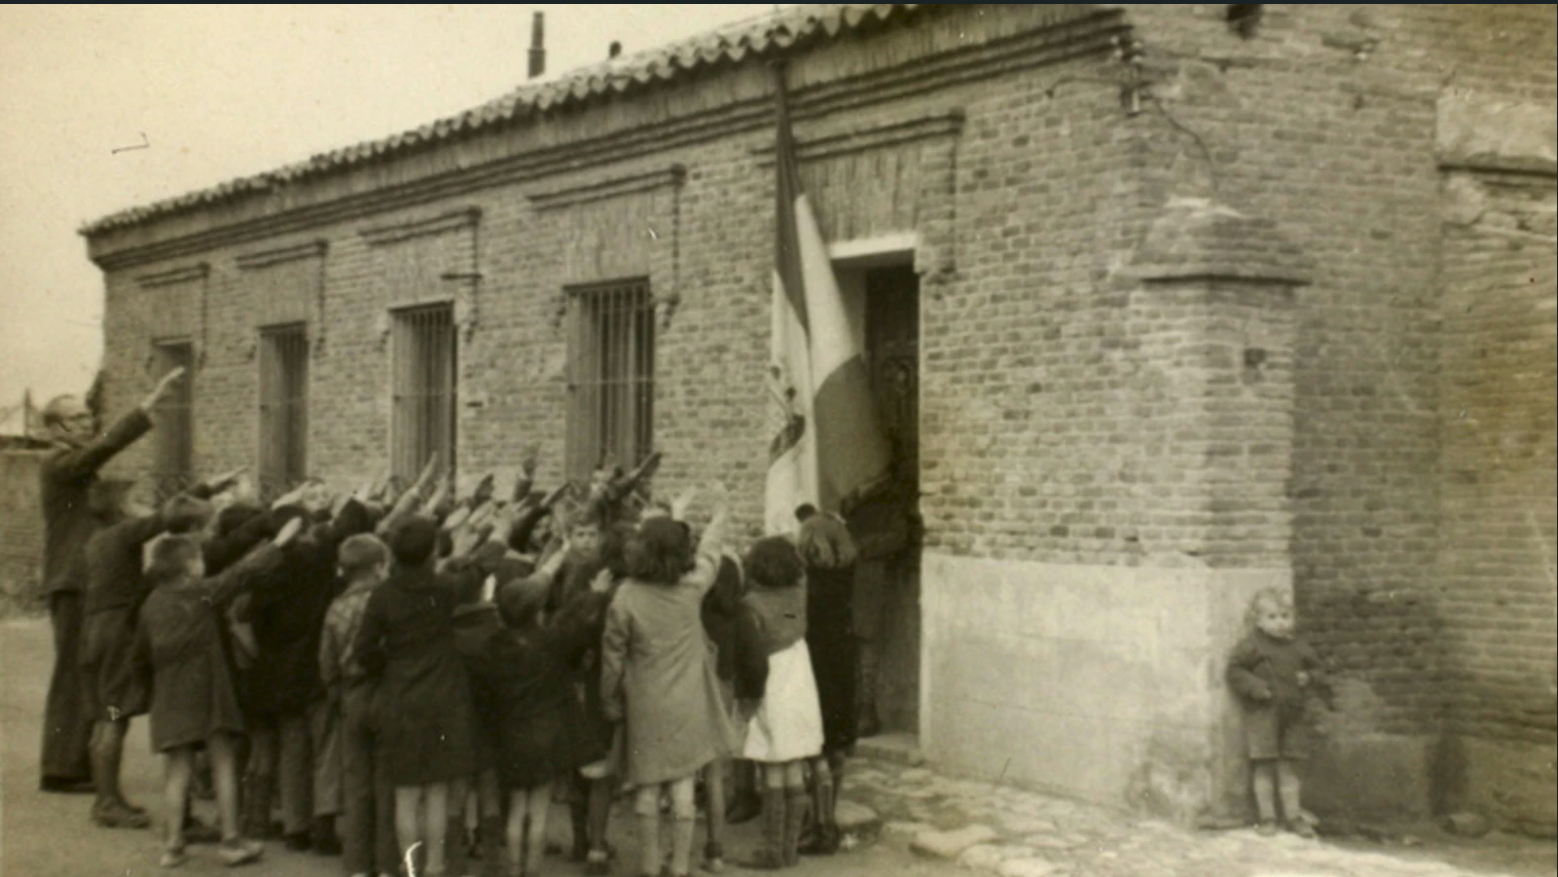
\includegraphics[width=\textwidth]{foto6}
                \caption{Kids singing \textit{"Cara al Sol"}}
                \label{fig:1}
            \end{subfigure}
        \end{minipage}
    \begin{minipage}{.45\linewidth}
        \begin{subfigure}[t]{1.1\linewidth}
            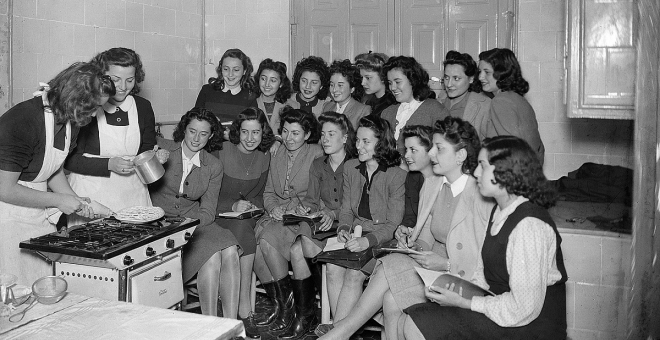
\includegraphics[width=\textwidth]{foto3}
            \caption{Women taking cooking classes}
            \label{fig:2}
        \end{subfigure} \\
        \begin{subfigure}[b]{1.1\linewidth}
            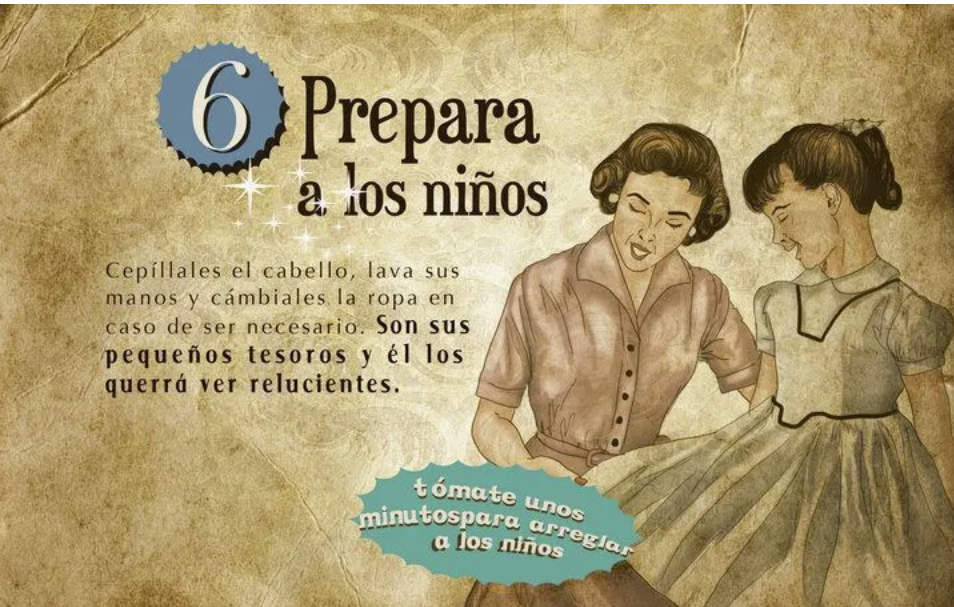
\includegraphics[width=\textwidth]{foto4}
            \caption{\textit{"Prepare the kids"}}
            \label{fig:2}
        \end{subfigure} 
    \end{minipage}
   % \caption{ }
\end{figure}
\end{frame}

\begin{frame}
\begin{figure}
    %\centering
 \begin{minipage}{.465\linewidth}
        \begin{subfigure}[t]{1\linewidth}
            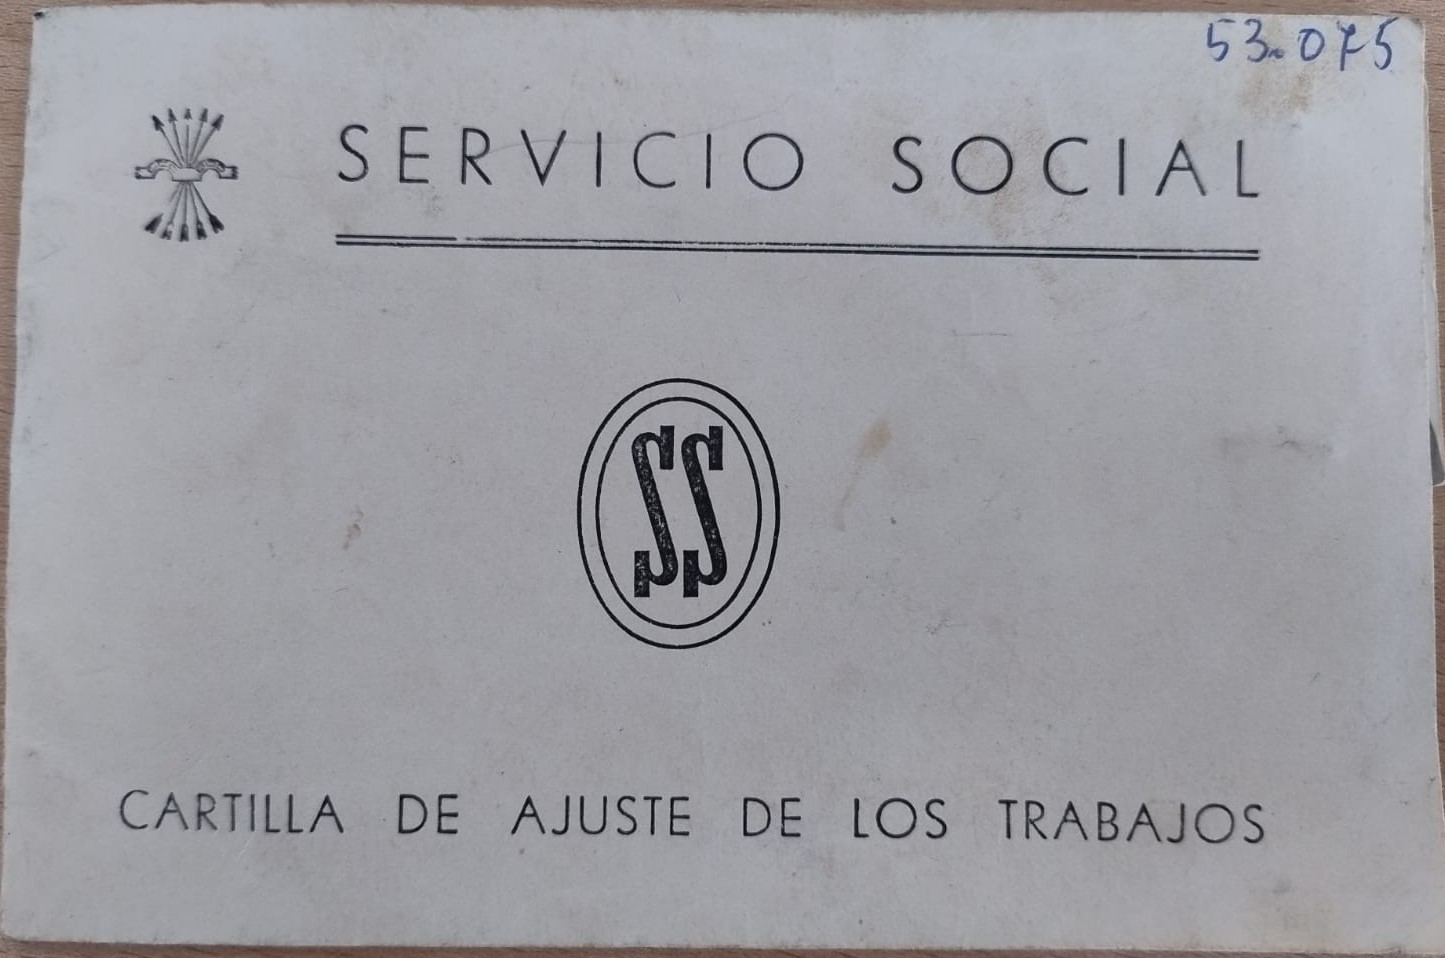
\includegraphics[width=\textwidth]{sf4}
            %\caption{Women taking cooking classes}
            \label{fig:2}
        \end{subfigure} \\
        \begin{subfigure}[b]{1\linewidth}
            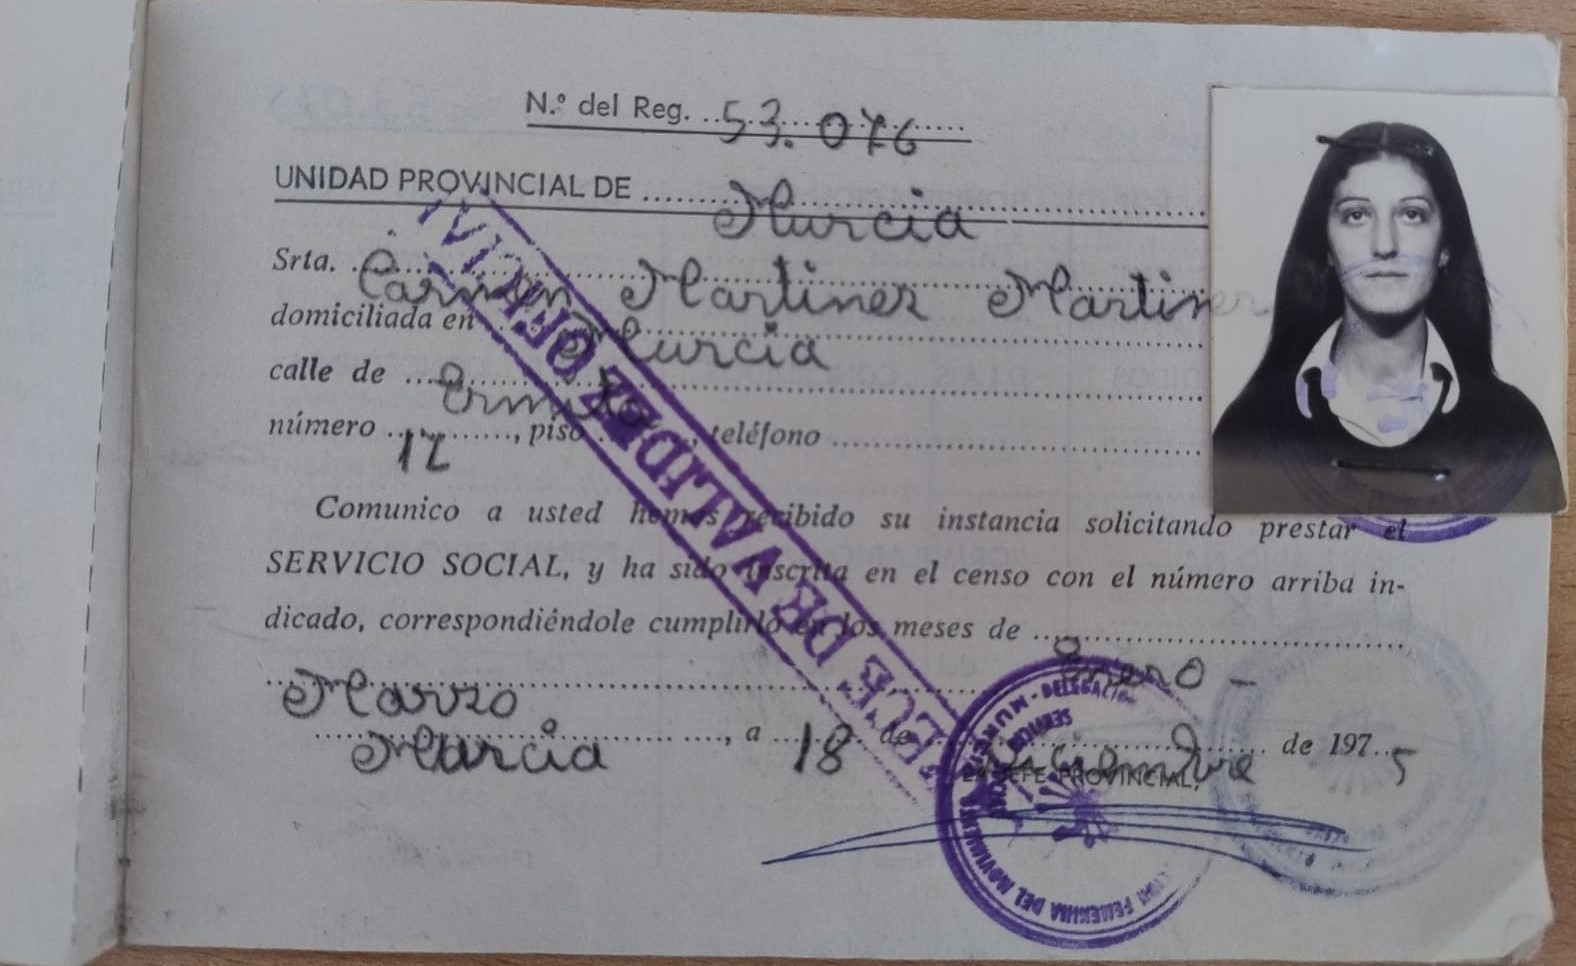
\includegraphics[width=\textwidth]{sf3}
            %\caption{\textit{"Prepare the kids"}}
            \label{fig:2}
        \end{subfigure} 
    \end{minipage}
    \begin{minipage}{.45\linewidth}
        \begin{subfigure}[t]{1\linewidth}
            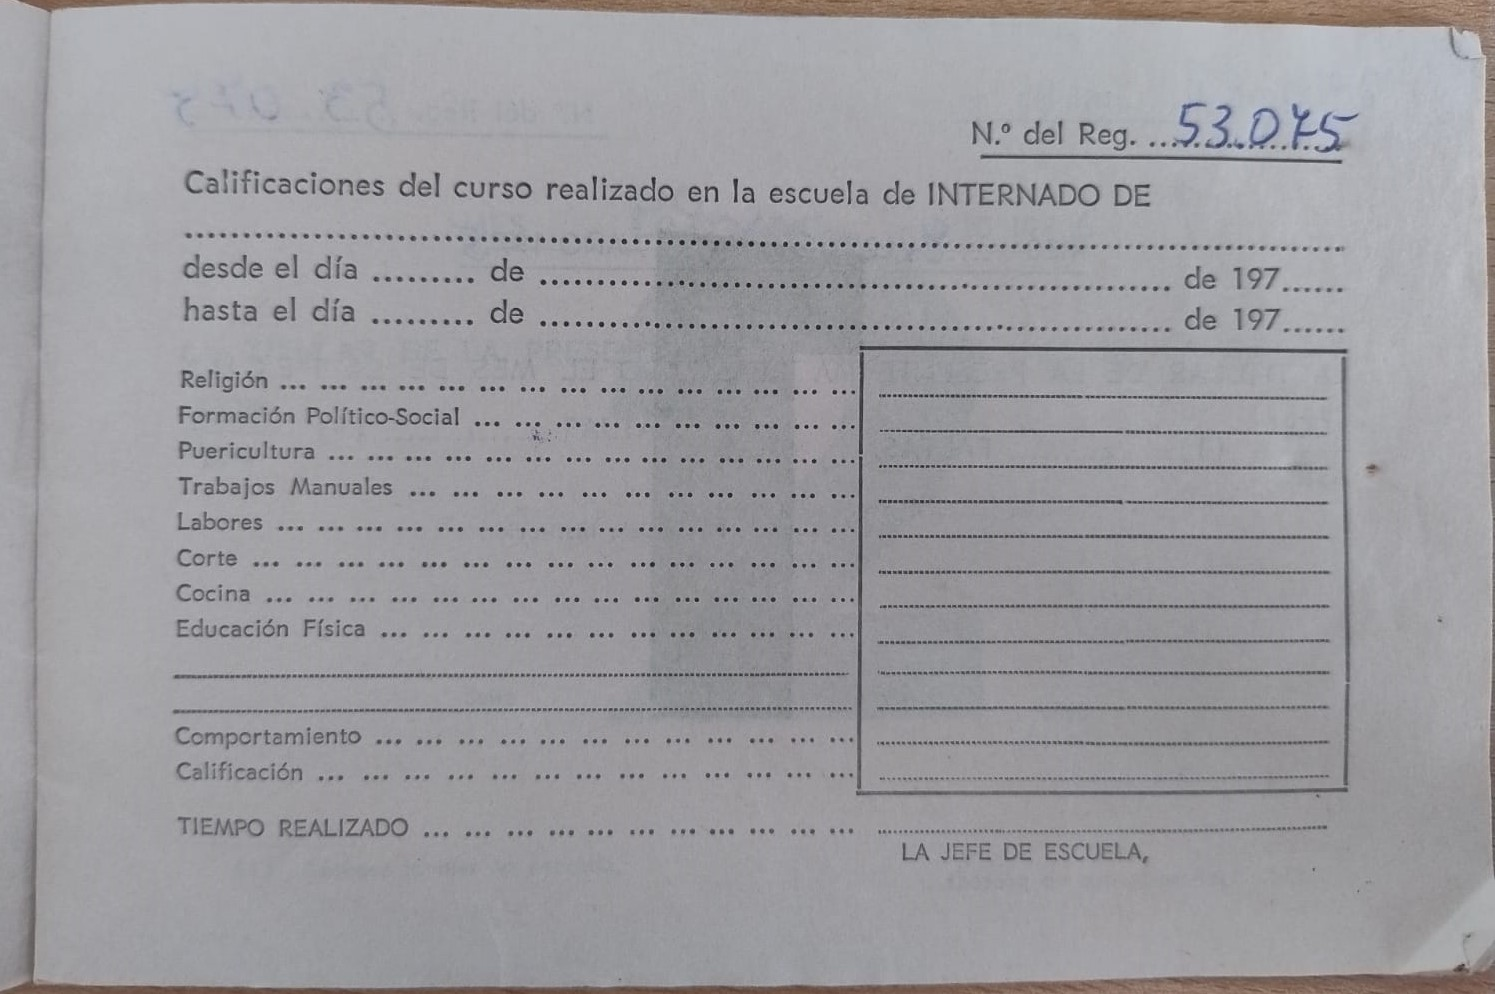
\includegraphics[width=\textwidth]{sf2}
            %\caption{Women taking cooking classes}
            \label{fig:2}
        \end{subfigure} \\
        \begin{subfigure}[b]{1\linewidth}
            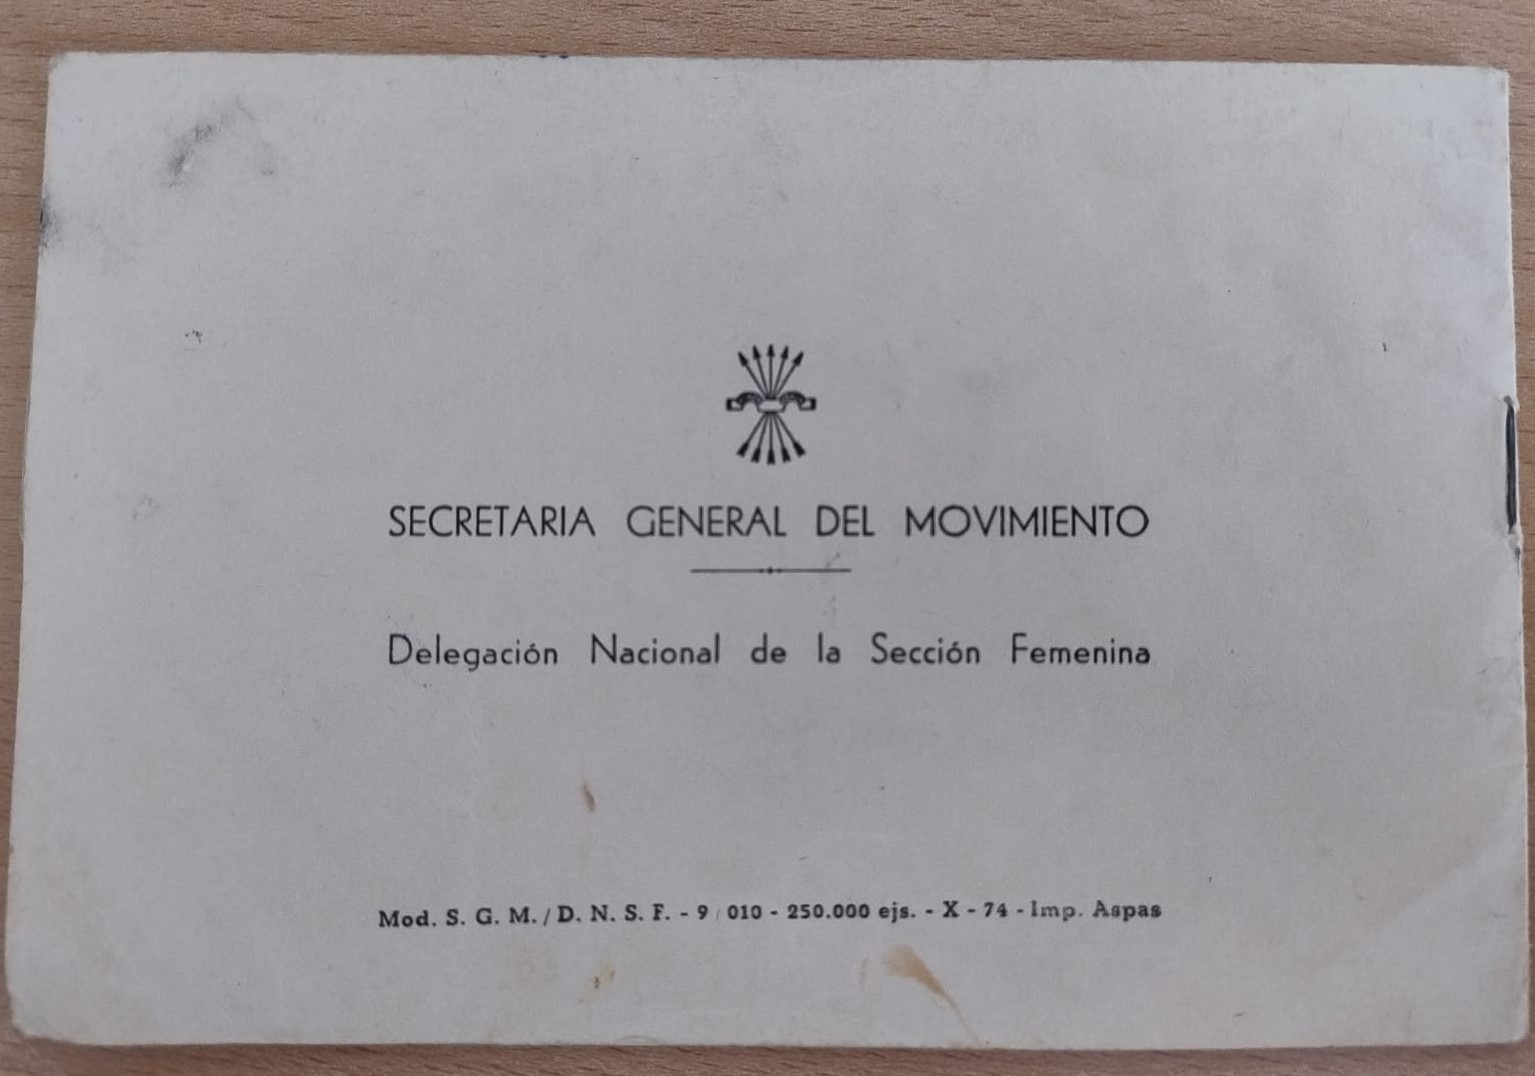
\includegraphics[width=\textwidth]{sf1}
            %\caption{\textit{"Prepare the kids"}}
            \label{fig:2}
        \end{subfigure} 
    \end{minipage}
   % \caption{ }
\end{figure}
\end{frame}
 %%%%%%%%%%%%%%%%%%%%%%%%%%%%%%%%%%%%%%%%%%%%%%%%%%
 %%%%%%%%%%%%%%%%%%%%%%%%%%%%%%%%%%%%%%%%%%%%%%%%%%
\begin{frame}
\begin{figure}
    %\centering
            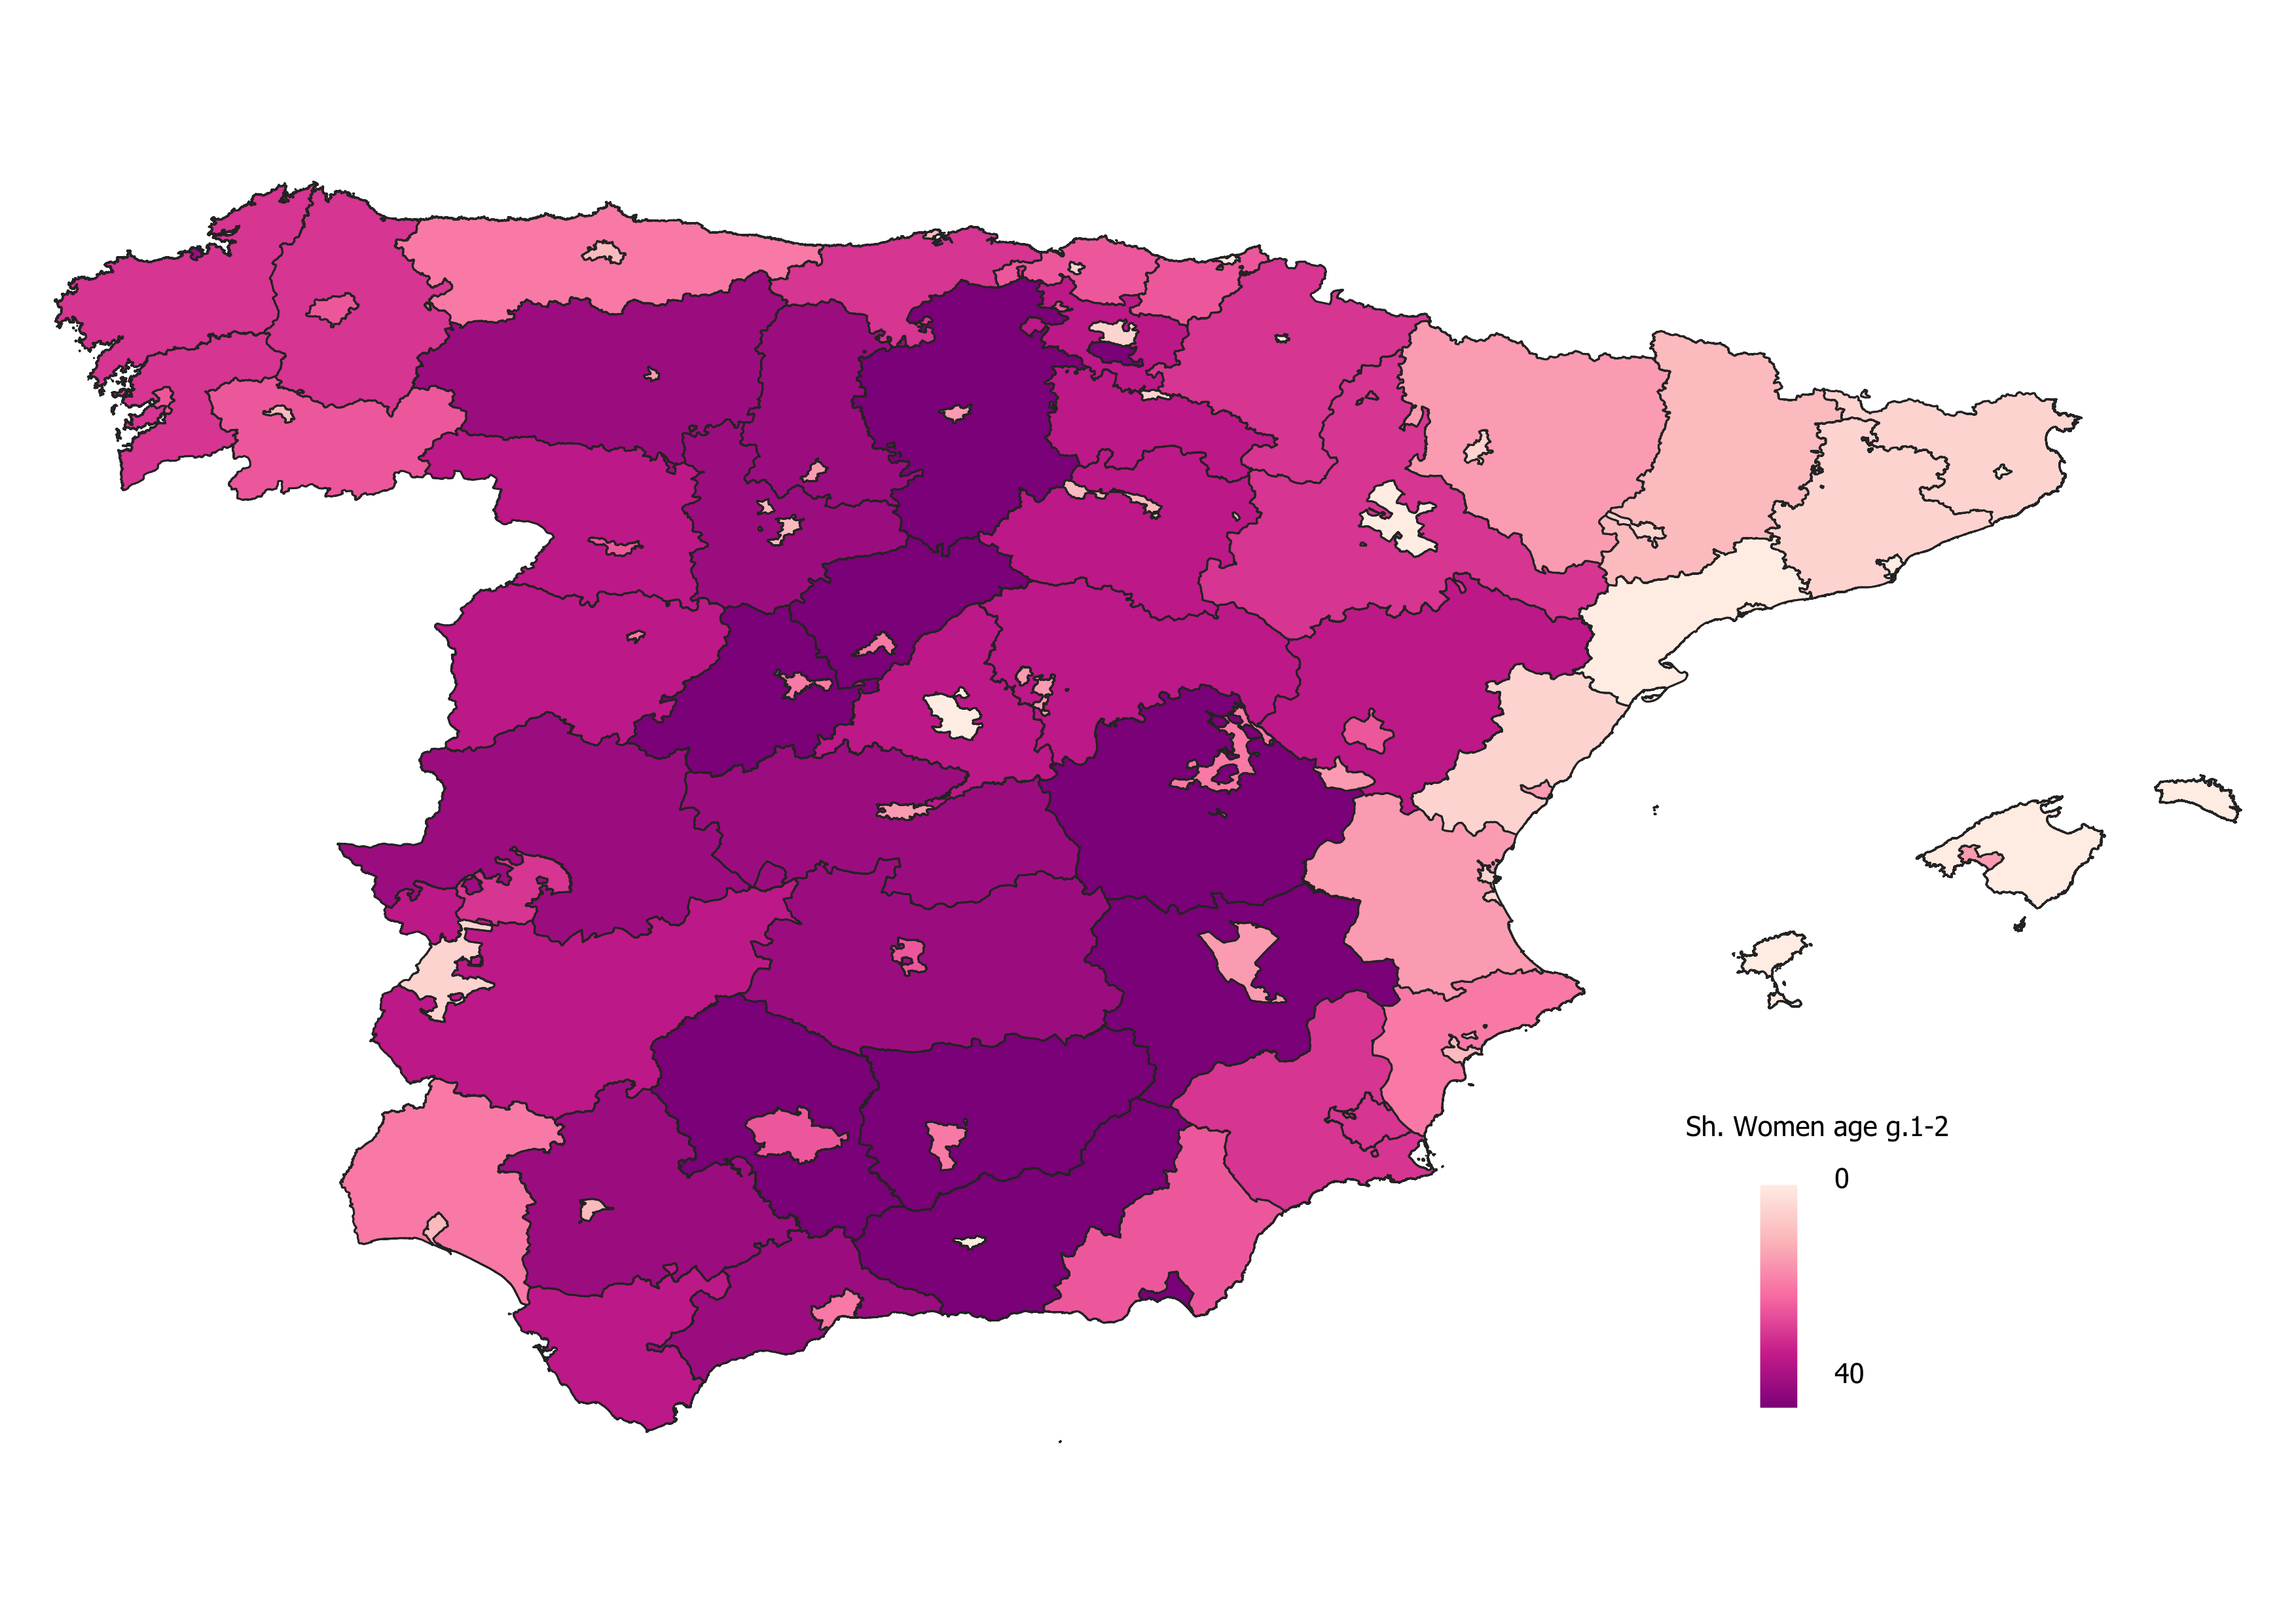
\includegraphics[width=0.8\textwidth]{desc_maps/popw.png}
            \caption{Share women age groups 1-2}
            \label{fig:2}
   % \caption{ }
\end{figure}
\end{frame}

 %%%%%%%%%%%%%%%%%%%%%%%%%%%%%%%%%%%%%%%%%%%%%%%%%%
\begin{frame}
\begin{figure}
    %\centering
            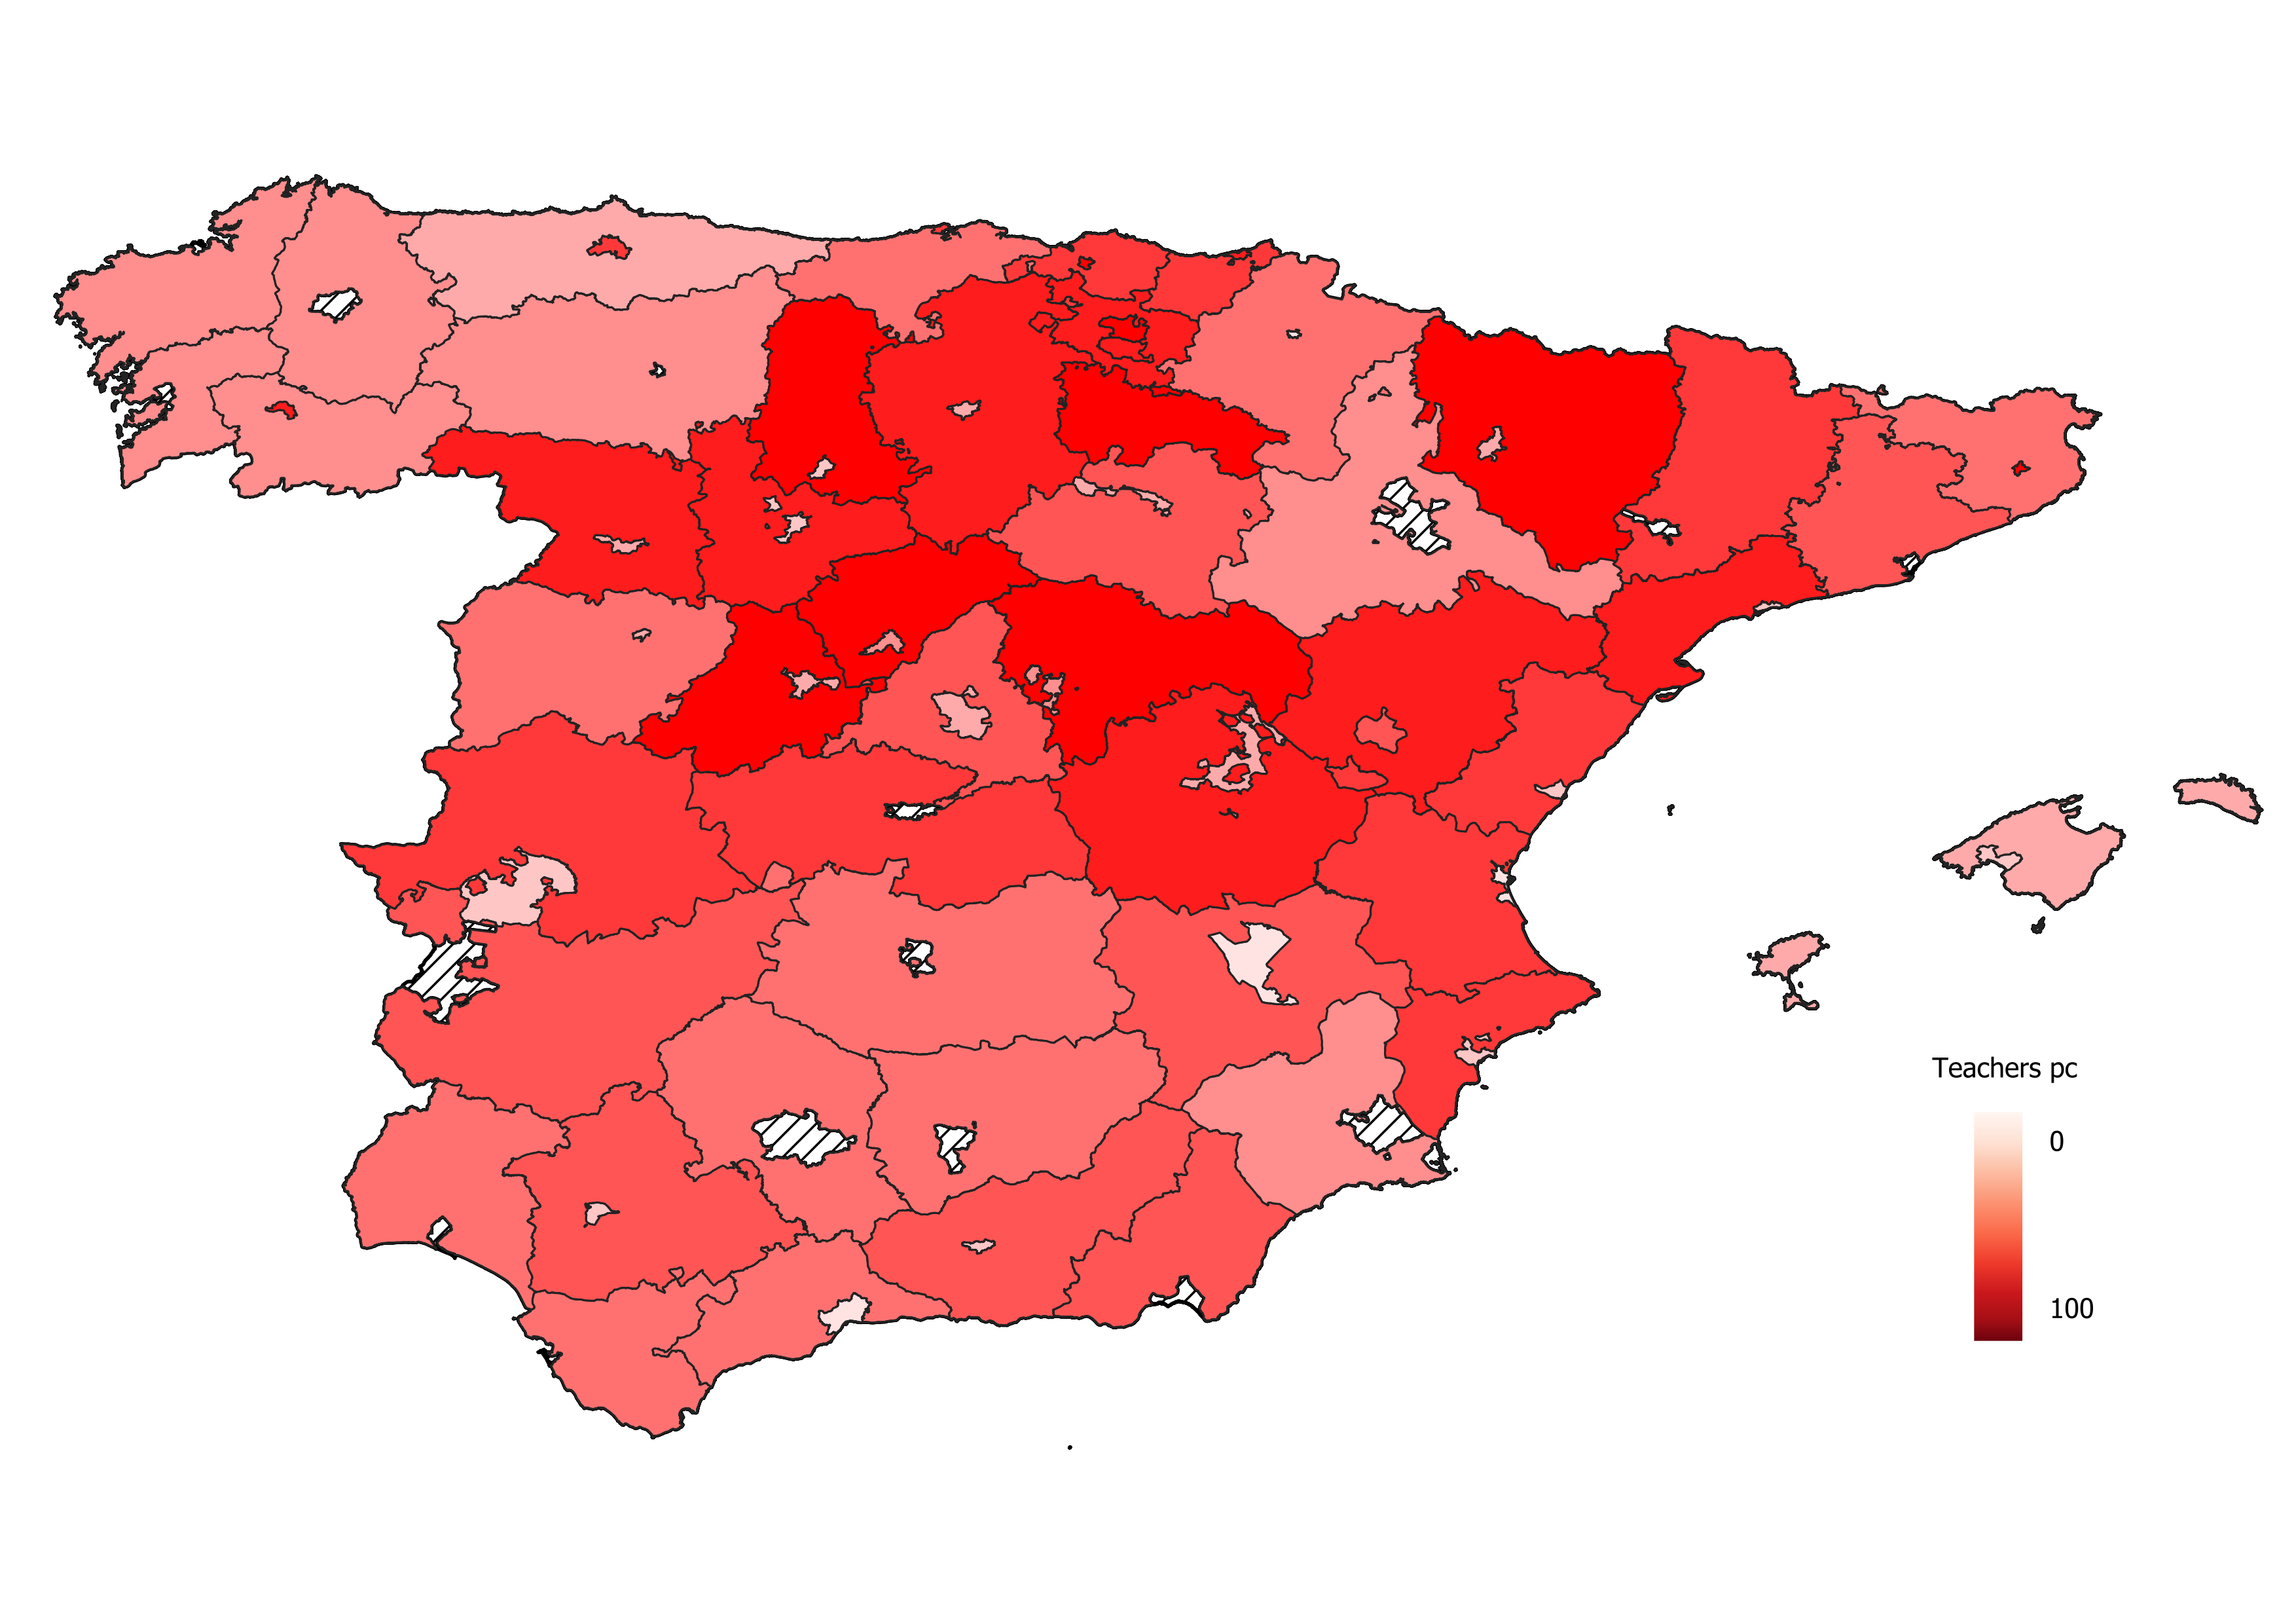
\includegraphics[width=0.8\textwidth]{desc_maps/teacherspc.png}
            \caption{Teachers pc}
            \label{fig:2}
   % \caption{ }
\end{figure}
\end{frame}
%%%%%%%%%%%%%%%%%%%%%%%%%%%%%%%%%%%%%%%%%%%%%%%%%%
\begin{frame}
\frametitle{Motivation}
\begin{itemize}
	   \item Demographic winter and policies that try to mitigate it
    \begin{itemize}
        \item 
    \end{itemize}
\end{itemize}
	
	
    
\end{frame}
 

%%%%%%%%%%%%%%%%%%%%%%%%%%%%%%%%%%%%%%%%%%%%%%%%%%
\begin{frame}
\frametitle{What we do}
\centering
\begin{itemize}
 \item 
\end{itemize}
\end{frame}

%%%%%%%%%%%%%%%%%%%%%%%%%%%%%%%%%%%%%%%%%%%%%%%%%%
\begin{frame}
\frametitle{What we find}
\begin{itemize}
	\item  j
\end{itemize}
 \end{frame}

%%%%%%%%%%%%%%%%%%%%%%%%%%%%%%%%%%%%%%%%%%%%%%%%%%
\begin{frame}
\frametitle{Literature review}


\begin{itemize}
\item {\color{blue}Indoctrination by autocratic regimes}: Adena et al. (2015), Cantoni et al. (2017), Meriläinen and Mitrunen (WP2024)\\
\textit{Spain:} Lapuente and Saez (2013); Ortega and Silanes (2009); Balcells and Villamil (2020)
         
\item {\color{blue}Effects of Indoctrination on Fertility}: 	Bruckner and Schwandt (2013),	Fouka (2019), 	Bertocchi and Dimico (2017),	Campante and Chor (2012), Baudin and Stelter (WP 2023)


\end{itemize}

\end{frame}
%%%%%%%%%%%%%%%%%%%%%%%%%%%%%%%%%%%%%%%%%%%%%%%%%%
%%%%%%%%%%%%%%%%%%%%%%%%%%%%%%%%%%%%%%%%%%%%%%%%%%

\section{Background}

\begin{frame}
\frametitle{Historical Background}
\begin{itemize}
\item Civil War (1936-1939)
\item Primary Education Law under Franco rule (BOE 1945)
    \begin{itemize}
    \item Religious education
    \item Strong national spirit
    \item Mandatory use of the Spanish language
    \item Special primary education for \textbf{girls} that prepares them for home life, crafts, and domestic industries
    \item The role of teachers is subordinated to the supreme interests of the nation
    \item The school age is extended up to 15 years, with school attendance being compulsory
    \item Separation of sexes. {\footnotesize Kindergarten schools and coeducational schools will always be run by female teachers.}
    \end{itemize}
\end{itemize}
\end{frame}


%%%%%%%%%%%%%%%%%%%%%%%%%%%%%%%%%%%%%%%%%%%%%%%%%%
\begin{frame}
\frametitle{Historical Background: \textit{Primary Education Law (BOE 1945)}}
\begin{figure}
    %\centering
 \begin{minipage}{.465\linewidth}
        \begin{subfigure}[t]{1.3\linewidth}
            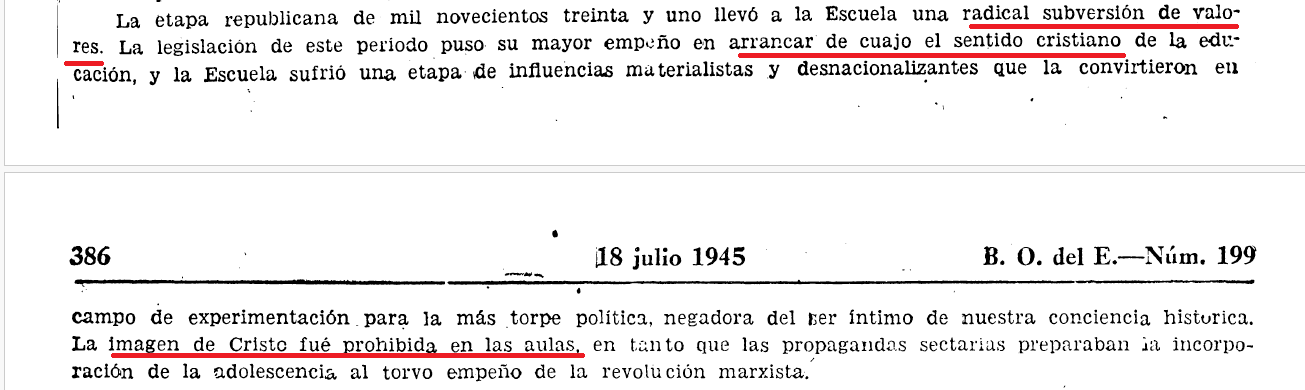
\includegraphics[width=\textwidth]{ley1.png}
            %\caption{Women taking cooking classes}
            \label{fig:2}
        \end{subfigure} 
    \end{minipage}
    \begin{minipage}{.45\linewidth}
        \begin{subfigure}[t]{1.2\linewidth}
            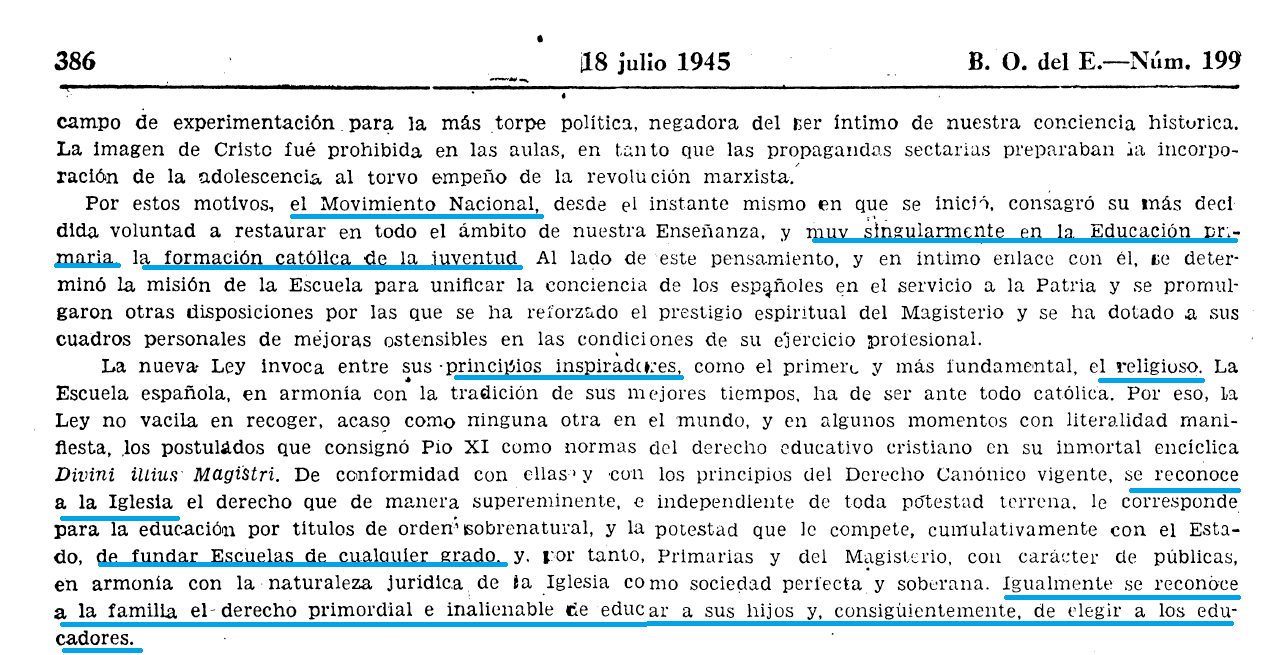
\includegraphics[width=\textwidth]{ley2.png}
            %\caption{Women taking cooking classes}
            \label{fig:2}
        \end{subfigure}
    \end{minipage}
   % \caption{ }
\end{figure}
\end{frame}


%%%%%%%%%%%%%%%%%%%%%%%%%%%%%%%%%%%%%%%%%%%%%%%%%%
\section{Data}
\begin{frame}
\frametitle{Data sources}
 
Panel data for 55 years (1930-1985). Unit of observation: capital of province and rest of province
\begin{itemize} \footnotesize
\item Population censuses from 1930 to 1970: number of inhabitants by age and gender
\item Fertility and wedding outcomes: Natural movement of the population- National  Institute of Statistics \textit{(INE)}
\item Teachers: General Archive of the Administration
\item Channels: Center for Sociological Research \textit{(CIS)}
\end{itemize}
\end{frame}
%%%%%%%%%%%%%%%%%%%%%%%%%%%%%%%%%%%%%%%%%%%%%%%%%%
\begin{frame}
\frametitle{Map }
 
\end{frame}

%%%%%%%%%%%%%%%%%%%%%%%%%%%%%%%%%%%%%%%%%%%%%%%%%%
\begin{frame}
\frametitle{Distribution of population by age groups}
\begin{figure}
    \centering
 \begin{minipage}{.46\linewidth}
        \begin{subfigure}[l]{1.2\linewidth}
            
\includegraphics[width=\textwidth]{gr_age/men.png}
            \caption{Male population}
            \label{fig:2}
        \end{subfigure} \\
    \end{minipage}
    \begin{minipage}{.45\linewidth}
              \begin{subfigure}[r]{1.2\linewidth}
            
\includegraphics[width=\textwidth]{gr_age/women.png}
            \caption{Female population}
            \label{fig:2}
        \end{subfigure} 
    \end{minipage}
   % \caption{ }
\end{figure}
\end{frame}
%%%%%%%%%%%%%%%%%%%%%%%%%%%%%%%%%%%%%%%%%%%%%%%%%%
\begin{frame}
\frametitle{Empirical Strategy}
 \begin{equation}\label{main_eq}
\begin{split} 
\small
y_{it} =\beta_0+ \beta_1 Post+\beta_2  \textit{Sh. Pop treated}_{i,1930}+\beta_3  \textit{Sh.  Teachers}_{i}+\\ 
+ \beta_4  \textit{Sh. Pop treated}_{i,1930} \times  \textit{Post}_{i} + \beta_5  \textit{Sh. Teachers}_{i,1930} \times  \textit{Post}_{i}+ \\
\beta_5  \textit{Sh. Pop treated}_{i,1930} \times  \textit{Sh. Teachers}_{i,1930} +\\
+\beta_7  \textit{Sh. Pop treated}_{i,1930} \times  \textit{Sh. Teachers}_{ip} \times Post+\Gamma_i+ \tau_t
\end{split}
\end{equation}

\begin{itemize}
\small
\item  $i$ and $t$ denotes an administrative unit  and   year
\item $y_{it}$ = birth rate (or number of weddings)=$\frac{\# births}{\text{Pop. Fertile age 1940}}$
\item $Post_{it}= \mathbbm{1} \{1945\}$ 

\item $\textit{Sh. Pop treated}_{i,1940}$ is the population share with 0-5 years old in 1940 

\item $\textit{Sh. Teachers}_{i,1930}$ is... 
\end{itemize}


\end{frame}
%%%%%%%%%%%%%%%%%%%%%%%%%%%%%%%%%%%%%%%%%%%%%%%%%%
\begin{frame}
\frametitle{Descriptive: \textit{Female population}}
\begin{figure}
    \centering
            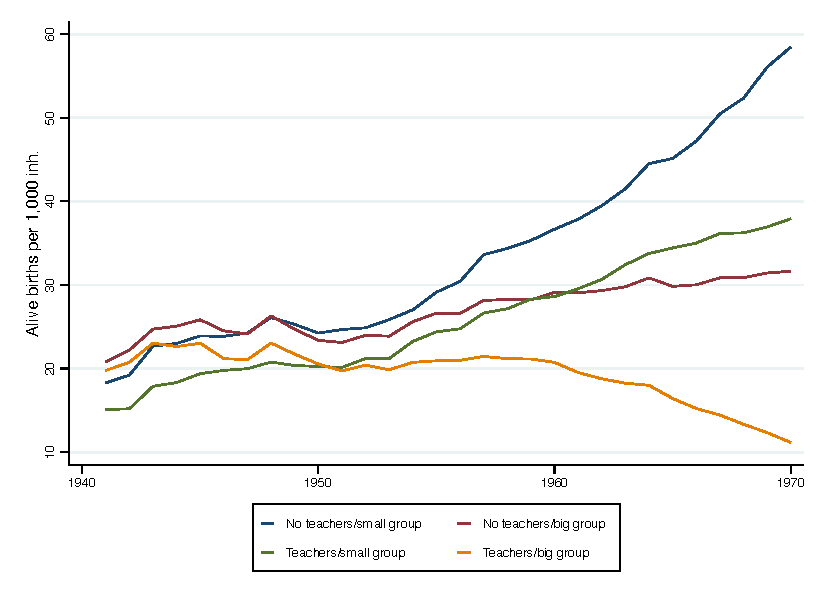
\includegraphics[width=0.9\textwidth]{Results/desc_1940_female.pdf}    
    \caption{ }
\end{figure}
\end{frame}
%%%%%%%%%%%%%%%%%%%%%%%%%%%%%%%%%%%%%%%%%%%%%%%%%%

%%%%%%%%%%%%%%%%%%%%%%%%%%%%%%%%%%%%%%%%%%%%%%%%%%

 %%%%%%%%%%%%%%%%%%%%%%%%%%%%%%%%%%%%%%%%%%%%%%%%%%

 \section{Results}
 \begin{frame}
\begin{center}
\textbf{{\LARGE RESULTS}}
\thispagestyle{empty}
\addtocounter{framenumber}{-1} % do not page count
\end{center}
\end{frame}
%%%%%%%%%%%%%%%%%%%%%%%%%%%%%%%%%%%%%%%%%%%%%%%%%%
\begin{frame}
\frametitle{Event study: birth rate \textit{Female population}}
\begin{figure}
    \centering
            \includegraphics[width=0.9\textwidth]{}    
    \caption{ }
\end{figure}
\end{frame}
%%%%%%%%%%%%%%%%%%%%%%%%%%%%%%%%%%%%%%%%%%%%%%%%%%
\begin{frame}
\frametitle{Event study: birth rate \textit{Male population}}
\begin{figure}
    \centering
            \includegraphics[width=0.9\textwidth]{}    
    \caption{ }
\end{figure}
\end{frame}
%%%%%%%%%%%%%%%%%%%%%%%%%%%%%%%%%%%%%%%%%%%%%%%%%%
\begin{frame}
\frametitle{Event study: weddings \textit{Female population}}
\begin{figure}
    \centering
            \includegraphics[width=0.9\textwidth]{}    
    \caption{ }
\end{figure}
\end{frame}
%%%%%%%%%%%%%%%%%%%%%%%%%%%%%%%%%%%%%%%%%%%%%%%%%%
\begin{frame}
\frametitle{Placebo }
\begin{itemize}
    \item Different age groups in 1940
    \item Same age group from census 1930
\end{itemize}
\end{frame}
%%%%%%%%%%%%%%%%%%%%%%%%%%%%%%%%%%%%%%%%%%%%%%%%%%
\begin{frame}
\frametitle{Conclusion}
\begin{itemize}
    \item 
    \item 
\end{itemize}
\end{frame}
 \end{document} 
 %%%%%%%%%%%%%%%%%%%%%%%%%%%%%%%%%%%%%%%%%%%%%%%%%%
